\documentclass[12pt,a4paper]{article}
\usepackage[utf8]{inputenc}
\usepackage[english]{babel}
\usepackage{amsmath}
\usepackage{amsfonts}
\usepackage{amssymb}
\usepackage{graphicx}
\graphicspath{ {./graphics/} }

\usepackage[top=1.5in, bottom=1in, left=1in, right=1in]{geometry}


\usepackage{float}

\usepackage{tikz}
\usetikzlibrary{arrows,automata, positioning,calc,shapes.geometric}

% header
\usepackage{fancyhdr}
\pagestyle{fancyplain}
\fancyhf{}
\lhead{ \fancyplain{}{Lukas Schwartz \& Aitor Miguel } }
\rhead{ \fancyplain{}{AI1 - 1. Semester MSc Robot Systems} }
\cfoot{ \fancyplain{}{\thepage} }

% make tables prettyer
\def\arraystretch{1.3}

\usepackage{todonotes}

\begin{document}

\begin{titlepage}
	\centering
%	\includegraphics[width=0.15\textwidth]{example-image-1x1}\par\vspace{1cm}
	\vfill
	{\scshape\LARGE University of Southern Denmark\par}
	\vspace{1cm}
	{\scshape\Large AI1 Project \#1\par}
	{\scshape\large 1. Semester MSc Robot Systems\par}
	\vspace{1.5cm}
	{\huge\bfseries Sokoban Solver\par}
	\vspace{2cm}
	{\Large\itshape Aitor Miguel Blanco \& Lukas Chr. M. W. Schwartz \\ Group \#1 \par}
	\vfill
	supervised by\par
	xyz

	\vspace{2cm}

% Bottom of the page
	{\large 3$^{rd}$ December 2015 \par}
\end{titlepage}

\pagebreak

\tableofcontents

\pagebreak

\listoffigures

\listoftables

\pagebreak


\section{Introduction}

This project describes the creation of an autonomous brick sorter to sort red, green and blue Lego bricks into separate directions.
This is to be done using a slide to which there is attached a servo motor to control whether the brick is going to the left or right.
Furthermore this project considers the design of the circuits used for power supplies and   color detecting circuit.

For the control of the brick sorter a FPGA is used to control the system.
The project also requires the use of uTosNet to communicate with a computer.

This report is structured such that it first describes the hardware and schematics used.
Thereafter the program run on the FPGA is considered and finally a test of the system is conducted and a conclusion on the whole project is drawn.



%This way, the project can be easily divided in 6 different blocks,

%\begin{itemize}
%\item Power supply
%\item Light sensor.
%\item LED Control.
%\item Servo motor.
%\item PC communication.
%\item VHDL design.
%\end{itemize}
	

\pagebreak
\section{Physical Design}
To solve the sokoban problem a robot capable of performing simple tasks concerned with moving the can and itself around the game map are needed.
The behaviours the robot should be able to perform define how the robot should be formed in order to accomplish its task of solving the sokoban problem.

\subsection{System Behaviours}
The robot was decided to be build upon being able to execute simple behaviours.
The execution of the behaviours would then be controlled from the \textit{Brain},
this is illustrated in figure \ref{fig:behaviourSystem}.

% brain/behaviour diagram
\begin{figure}[H]
\center
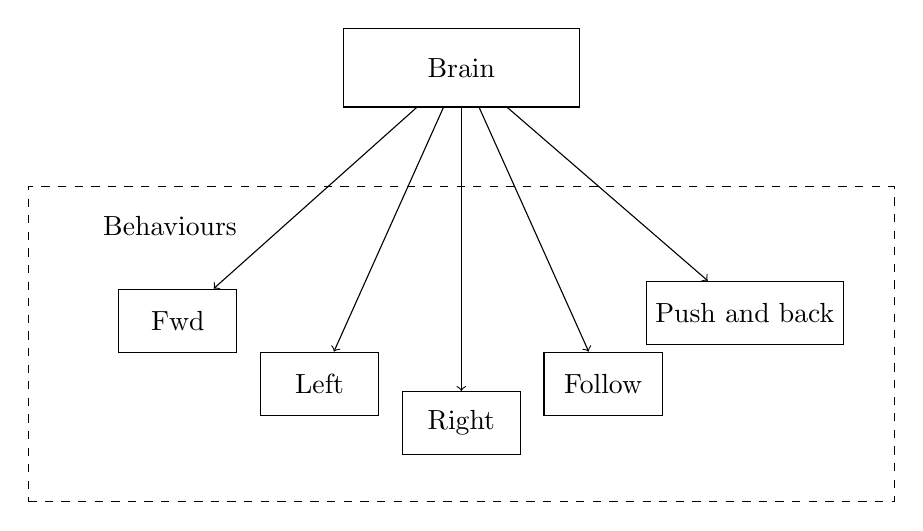
\begin{tikzpicture}[node distance=1cm]
%  behaviour box
\node[rectangle,draw,minimum width=11cm, minimum height=4cm, dashed, name=behaviour_box]  at (0,0) {};
\node[name=behaviour] at (-3.7,1.5) {Behaviours};

% Brain node 
\node[rectangle,draw,minimum width=3cm, minimum height=1cm, name=brain, above=of behaviour_box] {Brain};

% behaviours
\node[rectangle,draw,minimum width=1.5cm, minimum height=0.8cm, name=fwd] at (-3.6,0.3) {Fwd};
\node[rectangle,draw,minimum width=1.5cm, minimum height=0.8cm, name=left] at (-1.8,-0.5) {Left};
\node[rectangle,draw,minimum width=1.5cm, minimum height=0.8cm, name=right] at (0,-1.) {Right};
\node[rectangle,draw,minimum width=1.5cm, minimum height=0.8cm, name=follow] at (1.8,-0.5) {Follow};
\node[rectangle,draw,minimum width=1.5cm, minimum height=0.8cm, name=back] at (3.6,0.4) {Push and back};

% arrows inside 
\draw[->] (brain) -- (fwd) ;
\draw[->] (brain) -- (left) ;
\draw[->] (brain) -- (right) ;
\draw[->] (brain) -- (follow) ;
\draw[->] (brain) -- (back) ;
\end{tikzpicture}
\caption{Overview of the systems behaviours.}
\label{fig:behaviourSystem}
\end{figure}

Here the central unit, the \textit{Brain} is responsible for finding the solution to the sokoban problem by invoking the five behaviours.
The \textit{Brain} is hence a combination of both the computer processing the map offline and the Lego-robot online when using the offline generated data to solve the puzzle.

The behaviours are defined in table \ref{tab:behaviourExplained} and based on dividing the behaviours into simple tasks which are easy to program.

\begin{table}[H]
\center
\begin{tabular}{c|l}
Behaviour & Description \\ \hline
Fwd & Makes the robot go straight ahead in the next intersection. \\
Left / Right & The robot turns left/right in the next intersection. \\
Push and back & The robot pushes the can to the next intersection and \\ & goes back to the previous one. \\
Follow & Makes the robot follow the line till next intersection.
\end{tabular}
\caption{Behaviour table.}
\label{tab:behaviourExplained}
\end{table}

\todo[inline]{what about a separate push behaviour?}

With these five behaviours the robot should then be able to navigate around the map and when a tomato can is encountered, push it to its destination.
\subsection{Physical Structure}
The structure of the robot should allow the movement of the robot across the map. 
That means, the robot should have at least two motors to move in the plane of the circuit and a minimum of two light sensors to check its position referred to the black lines of the map and check when the robot has arrived to a crossroad.

The chosen motor configuration consist in the use of two motors that move two parallel wheels. 
This allows the robot to change the direction of the movement setting a different motor speed on each motor.

\todo[inline]{support? using the 3rd line sensor.}

Two light sensors are used as seen in figure \ref{fig:robotscheme}. 
In the position control, the value of the sensors are compared and the robot is controlled having in mind that the value of the sensors should be the same when the robot is centred above the line.
When the value of both sensors are low, the robot is facing a crossroad.

The position of the light sensors is in the front of the robot, and the distance between them should be enough to correctly detect the line. 
This means the light sensors should be placed close to the edges of the line such that they both detect a part of the line.
Because of that the distance between them should be around the width of the line itself as shown in figure \ref{fig:robotscheme}.

\todo[inline]{sensor offset? variability? stability?}

\begin{figure}[H]
\includegraphics[width=10cm]{Fig2.png}
\centering
\caption{Scheme of the proposed configuration.}
\label{fig:robotscheme}
\end{figure}


To be able to push and guide the can across the map, the robot should have a proper tool that allows this task. 
The proposed design consist of two bars placed making an angle that allows the guide of the bottle when driving straight forward, as is shown in figure \ref{fig:robotscheme}.
This configuration allows catching the can even when its position is displaced, making the robot's job more easy.

Considering the rules of the game then the can is not permitted to be pushed left or right and because of that, no special design enabling this are required. 
The turning back behaviour is more difficult. 
%As the distance between the lines are short, the turn back should be done in a small place because the sensors should find the line before the crossroad.
The distance between the line intersections are short and the turn back has to happen in free space without interacting with the nearby placed cans.
At the same time, the robot should also finish the turn before reaching the new intersection, so the full length of the robot should be short enough to allow these movements.


The final build of the robot is seen in figure \ref{fig:robotImage}.

\begin{figure}[H]
\includegraphics[width=10cm]{Fig1.png}
\centering
\caption{Images of the built robot.}
\label{fig:robotImage}
\end{figure}

\subsection{Tests of the Robot Behaviours}
In order to test the functionality of the behaviours implemented each can be tested individually.
Nevertheless, a more robust way of testing the behaviours is combine them in certain test circuits that can be looped to check the reliability of these behaviours.
By building a more complex circuit to test, the different behaviours can be tested in different ways so the position of the robot changes before each of them.

This way, three different experiments have been executed:
First, a test to check the robot is able to find, follow and get a good position on a line after right and left turning. 
With this test we can test the follow line, and turning behaviours.
The circuit used in this test was a "8", that means, the robot should turn left 4 times and then right 4 times in a row, 
as shown in figure algo.

The second test executed has looked at the ability of the robot to go back in a intersection and turn to different directions after finding the previous intersection.
This test has been done running a circuit where the robot goes back, find the next intersection and goes back to the previous one. 
Then the robot turns in different directions each time, checking the response of all of them in different cases, as these directions are mixed.

Finally, a experiment with a can has been executed to test the robot hability to push and place correctly the can.
In this experiment, the robot has to use all the different behaviours to move the can from one position to another and then to the original position again.

Each of the three experiments have been executed starting with a full power battery and the circuit set for each one has been repeated 20 times in up to 10 trials without a battery change or charge.
The time needed to complete the 20 laps has been measured for each trial.
This allows us to determine too the fucionality and response of the robot in long runs.

About the light sensors, they have been tested apart with a built structure to measure their response to different light levels and test the efectivity of shielding these sensors.
The description of this experiment is attached in \_reftolightsensors.



\_\_\_\_\_\_\_\_\_\_\_\_\_\_\_\_\_\_\_\_\_\_\_\_\_\_\_\_\_\_\_\_\_\_\_\_\_\_\_\_\_\_\_\_

The position controller used in the line following algorithm can be tested by letting the robot drive along a line and record the error of the line sensors.
The smaller it is able to hold the error, the better it is.
Furthermore the line following can be tested with and without the tomato can to check the response when the robot has a load.

To test the turning behaviours the robot can be told to drive in a square and if it is able to maintain the same square, the turning function works.

\todo[inline]{turning both ways? dropping a can after a push?}

\subsubsection{Results}

The results of the different behaviour experiments are shown in tables \ref{1} \ref{2} and \ref{3}.



\pagebreak
\section{Software}
This section describes the software used to control the brick sorting system.
First the top module is described and from there the individual components are considered.

The main components and their interface is shown in figure \ref{fig:program_design}.
Apart from the shown connections in figure \ref{fig:program_design}, then a set of connections to transfer variables which can be set from the computer and the clock signal.


\begin{figure}[H]
\centering
\begin{tikzpicture}[node distance=1cm]
% FPGA border
\node[rectangle,draw,minimum width=9cm, minimum height=7cm, dashed, name=FPGA]  {};

% used to align the insides of FPGA
\node[rectangle,minimum width=5cm, minimum height=5cm, name=FPGAaligne] {};

% components of FPGA
\node[rectangle,draw,minimum width=3cm, minimum height=1cm, name=utos] at (FPGAaligne.-135) {uTosNet};
\node[rectangle,draw,minimum width=3cm, minimum height=1cm, name=ad] at (FPGAaligne.45) {\begin{varwidth}{4cm}AD-Converter\\ Communication\end{varwidth}};
\node[rectangle,draw,minimum width=3cm, minimum height=1cm, name=mc] at (FPGAaligne.0) {Motor Control};
\node[rectangle,draw,minimum width=3cm, minimum height=1cm, name=fsm] at (FPGAaligne.180) {FSM};
\node[rectangle,draw,minimum width=3cm, minimum height=1cm, name=color] at (FPGAaligne.135) {Color Detector};

% nodes outside FPGA
\node [left=of utos,name=pc] {PC};
\node [right=of ad,name=adc] {SPI};
\node [left=of color,name=rgb] {RGB(2:0)};
\node [right=of mc,name=servo] {Servo};

% arrows inside FPGA
\draw[<->] (utos) -- node[] {} (fsm) ;
\draw[<-] (color) -- node[above] {10 bit} (ad) ;
\draw[->] (fsm) --  node[above] {2 bit} (mc) ;
\draw[->] (color) -- node[left] {2 bit} (fsm) ;
 
% arrows connected to the outside of FPGA
\draw[<->] (utos) to[out=180, in=0] node[] {} (pc) ;
\draw[->] (adc) to[out=180, in=0] node[] {} (ad) ;
\draw[->] (color) to[out=180, in=0] node[] {} (rgb) ;
\draw[->] (mc) to[out=0, in=180] node[] {} (servo) ;
\end{tikzpicture}

\caption{FPGA Program Design.}
\label{fig:program_design}
\end{figure}



The components of figure \ref{fig:program_design} are responsible for the following tasks.

\paragraph*{FSM}
The \textit{FSM} component is the top module of the system.
It connects the remaining components functionality in order to sort the bricks depending on their color and communicate with the computer.

\paragraph*{Color Detector}
The \textit{Color Detector} is responsible for controlling the LEDs and use the data from the ADC to decide the color of the bricks passing through the system.
This way it is able to connect the light intensity values from the photo-diode and relate them to a specific color.
From there the data is used to decide which brick, if any, is passing the sensor.

\paragraph*{AD-converter Communication}
This component implements the SPI communication to the ADC and feeds this onwards to the \textit{Color Detector}.


\paragraph*{Motor Control}
The \textit{Motor Control} component is controlling the servo motor using an input signal, deciding which of three positions it should be in.
Either the left- or right-tray or the idle position.

\paragraph*{uTosNet}
UTosNet is the component supplied by SDU which implements the communication with the computer.
This component is hence created such that it is capable of transferring data of importance to the FPGA and change specific settings or gather data from such.








\end{document}